\section{Experimental results}\label{sec:results}

To give comparative results on the quality of the initialisation processes 
considered in this work, four well-known, categorical, labelled datasets ---
soybean (large), mushroom, breast cancer, and zoo animal --- will be clustered
by the \(k\)-modes algorithm with each of the initialisation processes using
their respective number of classes as the number of clusters. These datasets
have been chosen to fall in line with the established literature, and for their
relative sizes and complexities. Each dataset is openly available under the
\href{http://mlr.cs.umass.edu/ml/}{UCI Machine Learning
Repository}~\cite{Dua2019}, and their characteristics are summarised in
Table~\ref{tab:dataset_summary}.

\begin{table}[htbp]
    \resizebox{\textwidth}{!}{%
        \begin{tabular}{lrrrlrr}
\toprule
{} &  No. rows &  No. cols &  No. classes &  Missing values &  Adjusted no. rows &  Adjusted no. classes \\
\midrule
Breast cancer &       699 &        10 &            2 &            True &                683 &                     2 \\
Mushroom      &      8124 &        22 &            2 &            True &               5644 &                     2 \\
Soybean       &       307 &        35 &           19 &            True &                266 &                    15 \\
Nursery       &     12960 &         8 &            5 &           False &              12960 &                     5 \\
\bottomrule
\end{tabular}

    }\caption{A summary of the benchmark datasets.}\label{tab:dataset_summary}
\end{table}

Clustering algorithms are often evaluated based on their performance as a
classifier~\cite{%
    Arthur2007,Cao2009,Cao2012,Huang1998,Ng2007,Olaode2014,Schaeffer2007%
}. This is a fundamentally flawed approach --- especially given that
classification belongs to an entirely different branch of learning. Moreover,
doing so requires a number of assumptions about the topology of the data within
the metric space that is being considered~\cite{Memoli2011}. One such assumption
is that the classes recorded in the data are indeed separable objects like
clusters.

This analysis does not consider evaluative metrics related to classification
such as accuracy, recall or precision. Instead, only internal metrics are
considered such as the cost function defined in~\eqref{eq:cost}. This metric is
label-invariant and its values are comparable across the different
initialisation methods. Furthermore, the effect of each initialisation method on
the initial and final clusterings can be captured with the cost function. An
additional, and often useful, metric is the silhouette coefficient. This
measures the ratio between the intra-cluster cohesion and inter-cluster
separation of a particular clustering. Therefore, it could be used in a similar
way to reveal the effect of each initialisation method. Unfortunately, this
metric loses its intuition under the distance measure employed here.\

we will not follow this approach since our motivation is to compare the
quality of the clustering produced when using these initialisation methods. So,
for the purposes of measuring the performance of our various initialisation
methods as parts of a clustering algorithm, we will make use of internal metrics
that are independent of any external information such as a class labelling.
This family of metrics are built up from two characteristics of the clusters
found: cohesion and separation. Cluster cohesion is effectively the summed,
within-cluster variation or dissimilarity of its points, whereas a cluster's
separation is a sum of the distances between all points in the cluster and every
other point not in the cluster. In this analysis, we will make use of two
internal measures for cluster validity: our cost function from
Definition~\ref{def:cost} and the average silhouette coefficient, or silhouette
score, of our clustering, defined below. 

%\begin{definition}\label{def:silhouette}
%    Let \textbf{X} be a dataset and consider a clustering of \textbf{X} into
%    \(k\) parts, denoted by \(C = \left\{C_1, \ldots, C_k\right\}\). For each
%    \(X^{(i)} \in \textbf{X}\), we define the following two quantities:
%    \begin{itemize}
%        \item Let \(a\left(X^{(i)}\right)\) denote the average dissimilarity
%            between \(X^{(i)}\) and every other point in its cluster. Without
%            loss of generality, let \(X^{(i)} \in C_l\). Then:
%            \[
%                a\left(X^{(i)}\right) := \frac{1}{|C_l|} D\left(C_l,
%                X^{(i)}\right)
%            \]
%        \item Let \(b\left(X^{(i)}\right)\) denote the lowest average 
%            dissimilarity between \(X^{(i)}\) and all other points in each
%            cluster other than \(C_l\). That is:
%            \[
%                b\left(X^{(i)}\right) := \min_{l' \neq l} \left\{
%                \frac{1}{|C_{l'}|} D\left(C_{l'}, X^{(i)}\right) \right\}
%            \]
%    \end{itemize}
%
%With these quantities we define, for each point in our datset, their
%    \emph{silhouette coefficient}, denoted by \(s(X^{(i)})\):
%    \[
%        s(X^{(i)}) := \frac{b\left(X^{(i)}\right) -
%        a\left(X^{(i)}\right)}{\max\left\{a\left(X^{(i)}\right),
%        b\left(X^{(i)}\right)\right\}}
%    \]
%
%    The \emph{silhouette score} of a clustering \(C\) is simply the average of
%all the silhouette coefficients. Silhouette scores take value in the range
%\([-1, 1]\). Negative scores generally suggest that elements in the data have
%been mis-clustered since there exists a closer cluster centre than its own.
%Values around 0 indicate overlapping clusters, whereas silhouette scores close
%to 1 suggest well-separated and effective clusters.
%\end{definition}


\subsection{Results}\label{subsec:results}

In this section, two sets of results will be considered. The first are the more
classically seen tables of metrics defined above, and the latter are a
collection of plots showing the descent in the cost function of the \(k\)-modes
algorithm over time. In either case, results are generated using the Python
library \href{https://github.com/nicodv/kmodes}{\texttt{kmodes}} to which the
proposed method has been added as another initialisation method. The number of
clusters to be determined, \(k\), is chosen as the number of classes associated
with each dataset. Note that this value may not be optimal (as suggested by the
relatively low silhouette scores in most cases), and that the class variable is
not considered in the running of the algorithm.

\subsubsection{Metric results}

Each of the tables of results given below were obtained by running the
\(k\)-modes algorithm 25 times with each initialisation method on the dataset in
question. For each of these 25 runs, the simulation is seeded to make the
results reproducible.

At each run of the experiment the number of epochs to termination, the initial
and final costs, and the average silhouette score were recorded for the
clustering found. These metrics are summarised below in
Tables~\ref{tab:soybean_results}~\--~\ref{tab:zoo_animal_results} by their mean
and median values, and their standard deviation over the 25 runs.

\begin{table}
    \centering
    \resizebox{\textwidth}{!}{%
        \begin{tabular}{llllll}
\toprule
{} &      Initial cost &        Final cost &     Silhouette & No. iterations &          Time \\
\midrule
Cao      &  2220.48 (41.755) &  1423.28 (67.357) &  -0.01 (0.001) &   4.36 (0.898) &  0.69 (0.068) \\
Huang    &  1592.88 (74.713) &  1448.66 (62.399) &  -0.00 (0.001) &   4.20 (1.325) &  0.43 (0.099) \\
Matching &  1586.38 (57.090) &  1327.74 (35.361) &  -0.01 (0.002) &   4.28 (1.031) &  0.23 (0.016) \\
\bottomrule
\end{tabular}

    }
    \captionof{table}{Summative metric results for the soybean dataset with
    \(k=15\).}\label{tab:soybean_summary}\vspace{20pt}

    \resizebox{\textwidth}{!}{%
        \begin{tabular}{lllll}
\toprule
{} &         Initial cost &          Final cost & No. iterations &          Time \\
\midrule
Cao      &     20381.00 (0.000) &    20376.00 (0.000) &   2.00 (0.000) &  5.18 (0.647) \\
Huang    &  23437.06 (1353.506) &  22091.04 (760.220) &   3.06 (1.018) &  5.81 (1.404) \\
Matching &  22970.80 (1264.522) &  21839.24 (753.933) &   2.90 (0.953) &  2.77 (0.300) \\
\bottomrule
\end{tabular}

    }
    \captionof{table}{Summative metric results for the mushroom dataset with
    \(k=2\).}\label{tab:mushroom_summary}\vspace{20pt}

    \resizebox{\textwidth}{!}{%
        \begin{tabular}{lllll}
\toprule
{} &      Initial cost &        Final cost & No. iterations &          Time \\
\midrule
Cao      &   2178.00 (0.000) &   1955.00 (0.000) &   4.00 (0.000) &  0.33 (0.010) \\
Huang    &  2123.12 (92.805) &  2023.80 (49.390) &   2.58 (0.810) &  0.23 (0.047) \\
Matching &  2110.68 (87.670) &  2015.42 (40.354) &   2.72 (0.834) &  0.17 (0.022) \\
\bottomrule
\end{tabular}

    }
    \captionof{table}{Summative metric results for the breast cancer dataset
    with \(k=2\).}\label{tab:breast_cancer_summary}\vspace{20pt}

    \resizebox{\textwidth}{!}{%
        \begin{tabular}{lllll}
\toprule
{} &     Initial cost &       Final cost & No. iterations &          Time \\
\midrule
Cao      &   394.00 (0.000) &   284.00 (0.000) &   2.00 (0.000) &  0.04 (0.001) \\
Huang    &  334.44 (31.635) &  309.22 (31.662) &   2.22 (0.648) &  0.03 (0.006) \\
Matching &  342.30 (39.067) &  313.68 (34.028) &   2.32 (0.891) &  0.03 (0.006) \\
\bottomrule
\end{tabular}

    }
    \captionof{table}{Summative metric results for the zoo animal dataset with
    \(k=7\).}\label{tab:zoo_summary}
\end{table}

\subsubsection{Epoch costs}

The epoch-cost plots in this section were created by setting an initial seed for
each initialisation method and then running the \(k\)-modes algorithm 25 times.
Of these runs, the best set of costs is then chosen by their final cost and
plotted.

Note that in each figure, dotted lines indicate the established initialisation
methods whilst solid lines are used for the proposed method.

\begin{figure}
    \centering
    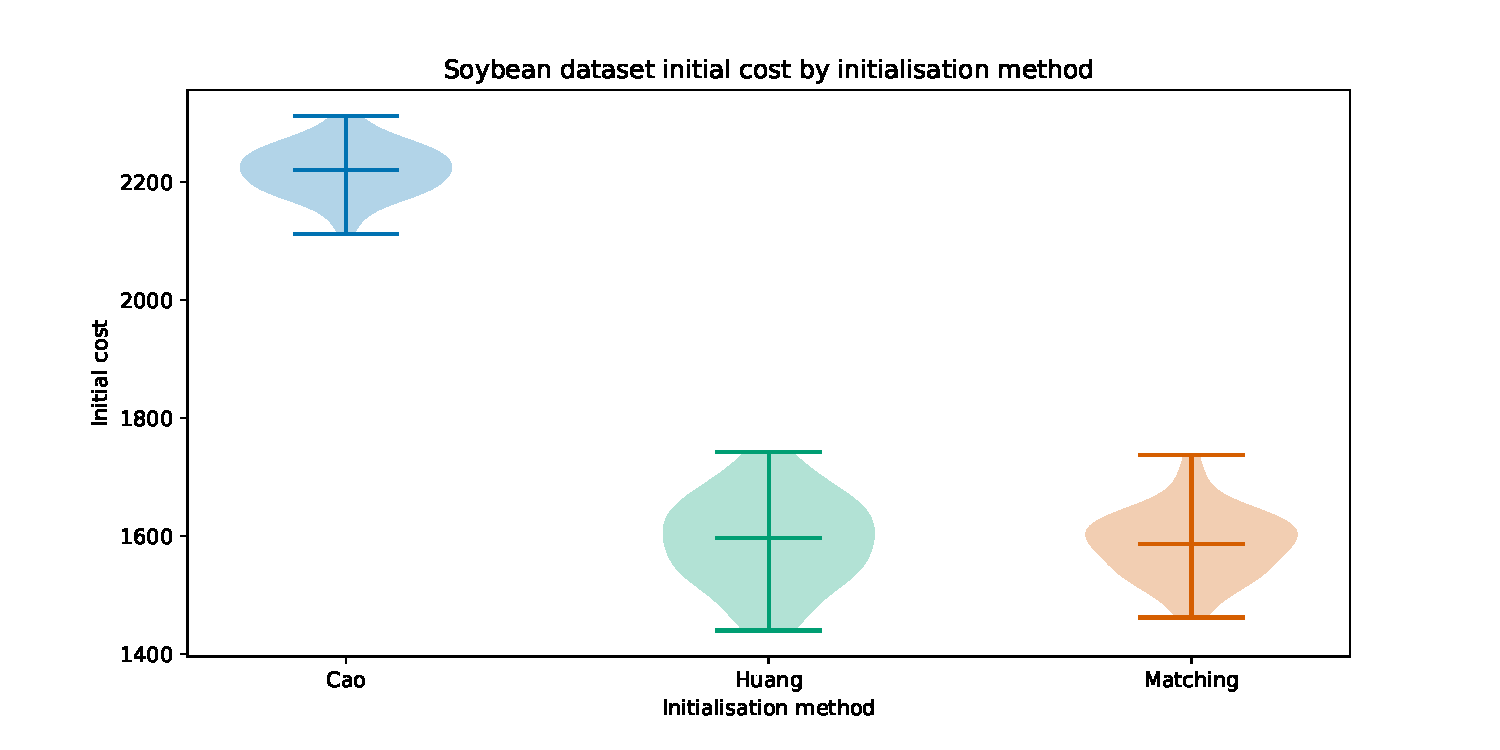
\includegraphics[width=\imgwidth]{%
        img/soybean_initial_cost_violinplot.pdf%
    }
\end{figure}

\begin{figure}
    \centering
    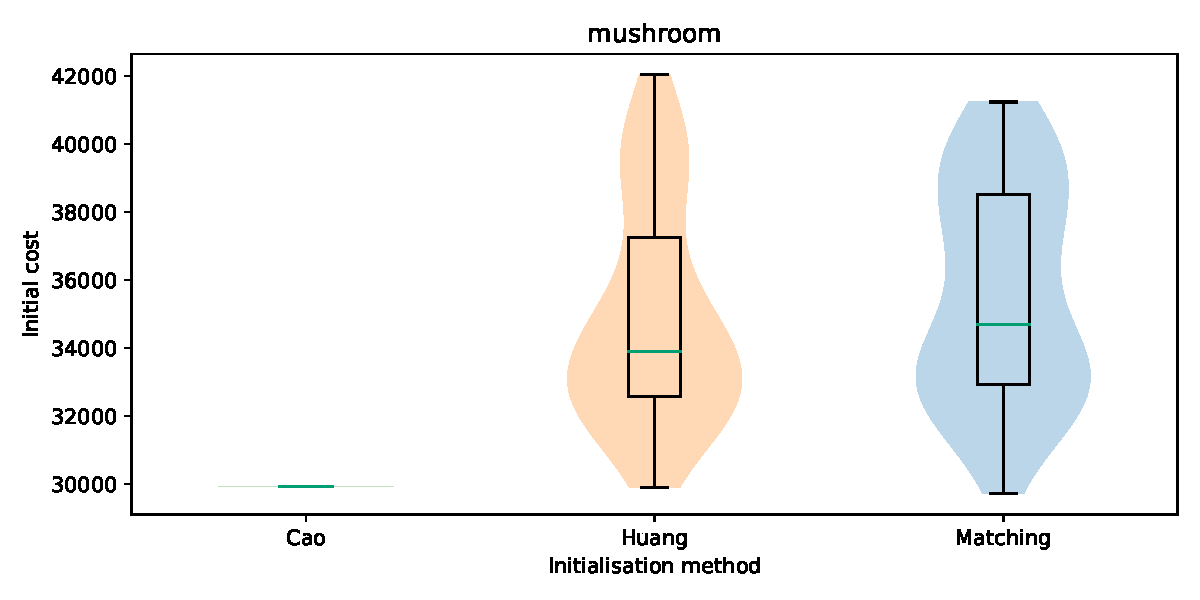
\includegraphics[width=\imgwidth]{%
        img/mushroom_initial_cost_violinplot.pdf%
    }
\end{figure}

\begin{figure}
    \centering
    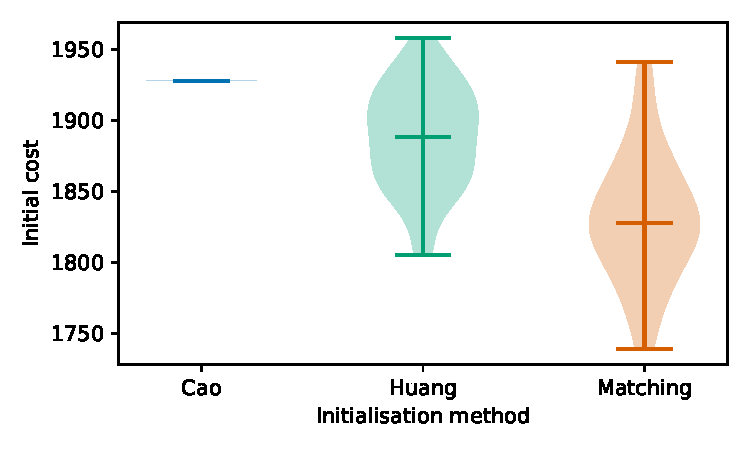
\includegraphics[width=\imgwidth]{%
        img/breast_cancer_initial_cost_violinplot.pdf%
    }
\end{figure}

\begin{figure}
    \centering
    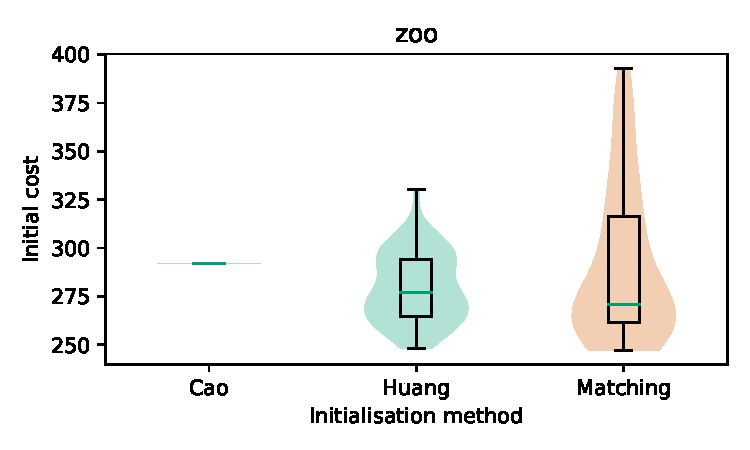
\includegraphics[width=\imgwidth]{%
        img/zoo_initial_cost_violinplot.pdf%
    }
\end{figure}
